\documentclass{bioinfo}
\copyrightyear{2019} \pubyear{2019}

\access{Advance Access Publication Date: Day Month 2019}
\appnotes{Application Note}

\begin{document}
\firstpage{1}

\subtitle{Genetic and population analysis}

\title[MPCC]{A Performant Matrix of Pearson$'$s Correlation Coefficient (MPCC) Calculations}
\author[Arends \textit{et~al}.]{
Danny Arends\,$^{\text{\sfb 1, $\dagger$}}$, 
Mitch Horton\,$^{\text{\sfb 2, $\dagger$}}$,
Chad Burdyshaw\,$^{\text{\sfb 2, $\dagger$}}$,
Christian Fischer\,$^{\text{\sfb 3}}$,
Pjotr Prins\,$^{\text{\sfb 3}}$,
Rob W. Williams\,$^{\text{\sfb 3, *}}$,
Glen Brook\,$^{\text{\sfb 2, *}}$}
\address{$^{\text{\sf 1}}$Z{\"u}chtungsbiologie und molekulare 
Genetik, Albrecht Daniel Thaer-Institut, Berlin, 10115, Germany \\
$^{\text{\sf 2}}$The Joint Institute for Computational Sciences, 
University of Tennessee, Oak 
Ridge, TN 37830, USA\\
$^{\text{\sf 3}}$Genetics, Genomics and Informatics, University 
of Tennessee Health Science Center, Memphis, TN 38163, USA.}

\corresp{$^\dagger$Contributed equally and should be considered 
joined first authors, $^\ast$To whom correspondence should be 
addressed.}

\history{Received on XXXXX; revised on XXXXX; accepted on XXXXX}

\editor{Associate Editor: XXXXXXX}

\abstract{\textbf{Motivation:} 
The work presented is motivated by GeneNetwork.org, which performs 
a matrix of Pearson$'$s Correlation Coefficient (PCC) calculations 
in the presence of missing data to find relationships between and 
among genotypes and phenotypes in mouse strains. The calculations 
are a bottleneck for moderate to large problem sizes. Calculating 
PCC is pervasive across bioinformatics, data analysis, 
phylogenetics, statistics, stochastics, and anthropology. Our 
approach can be used whenever a PCC matrix is computed.\\
\textbf{Results:} Our solution is a reformulation of the PCC algorithm 
such that the lion's share of the computation is done using matrix-matrix products and
achieves 4.3 TFlop/s in single precision (77\% of the theoretical 
peak) on a single Intel Xeon Gold 6148 CPU $@$ 2.4 GHz (Skylake) 
cpu. This translates to as much as a 100x speedup over the 
previous approach and is independent of the percentage of missing 
data.\\
\textbf{Availability:} Code is available for C\raise .8ex \hbox{$_{++}$} and The R Project for Statistical 
Computing, under an GPL-v3 licence  at \href{https://github.com/UTennessee-JICS/MPCC}{https://github.com/UTennessee-JICS/MPCC}\\
\textbf{Contact:} \href{rwilliams@uthsc.edu}{rwilliams@uthsc.edu} or 
\href{glenn-brook@tennessee.edu}{glenn-brook@tennessee.edu}\\
\textbf{Supplementary information:} Supplementary data are 
available at \textit{Bioinformatics} online.}

\maketitle

\section{Introduction}
Biology has driven innovation in statistics from the early days. Pearson, Fischer, 
Galton, and many other now famous statisticians were all working on biological 
problems. 
%The mathematical formula for Pearson$'$s correlation were derived by 
%Auguste Bravais in 1844. However, as Stigler's Law \citep{Stigler1980} dictates, 
%the name of the method credits Karl Pearson, who was building on ideas published 
%by Francis Galton in the 1880s.

\enlargethispage{12pt}

Pearson$'$s correlation is one of the most used algorithms in science. Its use is 
ubiquitous across all fields of science ranging from agriculture to zoology. Large 
scale computation of correlations are found in many areas of biology and 
bioinformatics. 

Genotype correlations are used to construct haplotypes, build genetic maps, and 
order markers within the genome. Furthermore, Pearson$'$s correlations are used in 
co-expression analysis \citep{Tesson:2010}, (genome wide) association analysis, 
reconstruction of genetic networks \citep{Fukushima:2013}, weighted correlation 
network analysis (WGCNA) \citep{Horvath:2008} and correlated trait locus (CTL) 
mapping \citep{Arends2016a}.

The BxD family is a panel of 150 recombinant inbred mice, and the BxD data collection 
consists of 7000 hand curated classical phenotypes, high-density genotypes, and over 
100 'omics' data sets. All BxD phenotype, genotype, and omics data is freely available on 
\href{https://genenetwork.org/}{GeneNetwork.org} \citep{Sloan2016}. GeneNetwork is an 
online platform for data storage and analysis, including Pearson$'$s correlation.

Computation of Pearson$'$s correlations in the R language for statistical computing 
\citep{R:2005} is provided by the $cor()$ function. It is implemented in C++ and is 
relatively performant when no missing data is present. In the presence of missing 
data, two strategies are used to deal with the missing data.

Consider the case where, for a set of individuals, pairwise correlation is done 
amongst the set of phenotypes for those individuals. Strategy 1 is to remove 
all individuals that contain any missing phenotype data. This is undesirable in 
biological data because often there are no individuals without at least some 
missing data. Strategy 2 handles missing data on a case by case basis, 
which significantly increases the algorithms runtime.

An additional issue with the $cor()$ function is the inability to, by default, use 
multi-threading. This limitation can be solved by using the $parallel$ library. 
However, not every end user has the ability to correctly setup the $parallel$ 
library, and the library uses a new R instance for each thread, adding significant 
computational overhead.
\vspace*{-5mm}
\begin{figure}[!t]
  \centerline{\includegraphics[width=235pt]{img/figure01.eps}}
  \vspace*{-7mm}
  \caption{
    Genotype to genotype correlation between genetic markers on chromosome 
    1 of the BxD family. Pairwise correlation between all 7321 marker was \textasciitilde{}6 times 
    faster using MPCC.
  }
  \label{fig:fig1}
  \vspace*{-5mm}
\end{figure}
\begin{figure}[!t]
  \centerline{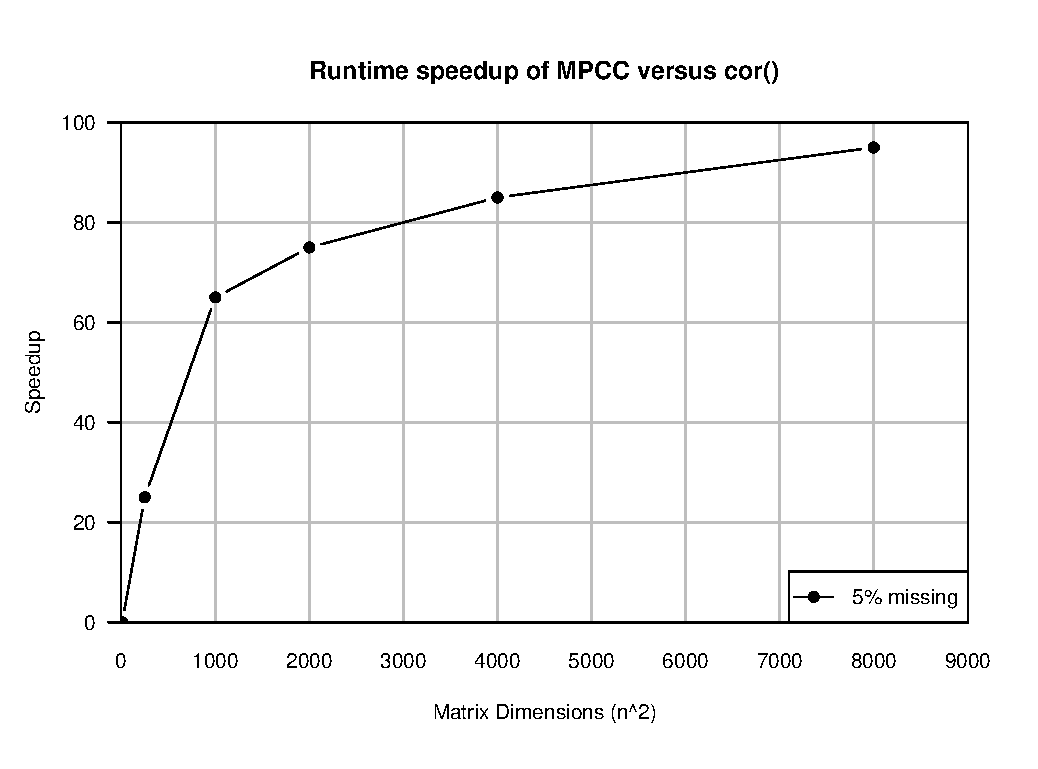
\includegraphics[width=235pt]{img/figure02.eps}}
  \vspace*{-7mm}
  \caption{
    Runtime speedup of MPCC versus the R $cor$ function shows 
    increasing speedup with growing matrix sizes. However, 
    speedup is negatively affected by increasing percentage of 
    missing data, because of increased computational load in the 
    missing data preparation step.
  }
  \label{fig:fig2}
  \vspace*{-5mm}
\end{figure}
\section{Approach}
\textbf{The Naive Version}\\
The Naive version of the MPCC algorithm was developed to be algorithmically identical 
to the R $cor()$ function (Supplement 1 - 'The Naive Version'). Multi-threading 
support without additional overhead is provided by OpenMP. The Naive version 
provides a fair multi-threaded baseline against the Matrix version. It also provides 
a multi-threaded fallback in R when no Intel\textregistered{} Math Kernel Library 
(Intel\textregistered{} MKL) is available.\\
\textbf{The Matrix Version}\\
The Matrix version reformulates the naive version of the PCC algorithm 
into a series of matrix-matrix products and element-wise matrix operations. 
Missing data is handled by a bit-masking approach implemented in C. 
Reformulation of the algorithm and our missing data strategy is described 
in detail in Supplement 1 - 'The Matrix Version' and 'Missing Data Bit-masking'. 
\vspace*{-5mm}
\begin{methods}
\section{Methods}
Two scenarios were designed to benchmark MPCC.\\
{\bf Scenario 1:} Pairwise correlation between genotypes of the BxD family. 
Genotype data in the BxD family is almost complete, with only a few heterozygous 
(missing) loci remaining, this scenario benchmarks MPCC versus $cor()$ when a limited 
amount of missing data is present.\\
{\bf Scenario 2:} Speedup computation of MPCC versus $cor()$ in the presence of a 
increasing amounts of missing data. Matrix sizes are increased in a step-wise fashion 
to increase computational load.
\end{methods}
\vspace*{-2mm}
\section{Results}
Both the Naive and Matrix versions provide R interfaces designed as a drop-in 
replacement for the $cor()$ function provided by R.

The Naive version using OpenMP to improve performance in comparison to the 
$cor()$ function provides a consistent 3.5x speedup (56 core Intel Xeon E5-2680 
v4 $@$ 2.40GHz - data not shown).

Using MPCC to compute genotype to genotype correlations (Fig \ref{fig:fig1}) leads to 
an \textasciitilde{}6x speedup compared to the $cor()$ function provided in R.

Multicore performance (40 cores) of MPCC compared to the $cor()$ function, shows up to a 
120 times reduction in runtime (Fig \ref{fig:fig2}). With increasing matrix sizes, 
the MPCC algorithm achieves an increasing speedup due to the increased arithmetic 
intensity of the algorithm. However, increasing the volume of missing data reduces the 
efficiency of MPCC due to preprocessing steps.
\vspace*{-5mm}
\section{Discussion}
The Matrix version heavily leverages the Intel\textregistered{} MKL to obtain 
maximum performance on Intel\textregistered{} systems. The performance of the 
matrix version is due in part to the high arithmetic intensity of the 
matrix-matrix product algorithm, on which it is based, and in 
part to the fact that the MKL matrix-matrix product algorithm is highly 
optimized for Intel architectures.  

The missing data approach (Supplement 1 - 'Missing Data Bit-masking') can be 
trivially generalized to other algorithms which rely on matrix-matrix multiplication.

Future work will investigate using OpenBLAS to provide a Free and Open-Source 
Software (FOSS) alternative to the Intel\textregistered{} MKL, as well as the 
feasibility of a GPU implementation.
\vspace*{-5mm}
\section{Conclusion}
Driven by demands in large data biology, computation of PCC was optimized. 
MPCC greatly reduces the existing bottlenecks for many fields faced with 
large problem sizes. The MPCC algorithm is much more efficient in its handling 
of missing data, a common issue in bioinformatics, since missing data is 
ubiquitous and leads to reduced performance.

A 120x speedup allows researchers to tackle many problems that could 
not have been attempted before. MPCC can be used by any language which 
allows calling C code. Furthermore, an R package with a drop-in 
replacement for the $cor()$ function is provided.
\vspace*{-5mm}
\section*{Funding}
We thank the support of the UT Center for Integrative and Translational Genomics, 
and funds from the UT-ORNL Governor's Chair, NIDA grant P30DA044223, NIAAA U01 
AA013499 and U01 AA016662.
\vspace*{-5mm}
\bibliographystyle{natbib}
\bibliography{main}

\end{document}
